\chapter{ResStock Workflow} \label{sec:workflow}
%% TONY converted https://resstock.readthedocs.io/en/latest/workflow_inputs/characteristics.html to LATEX. using "pandoc -f rst -t latex characteristics.rst > characteristics.tex"
%% TODO: LIXI: (From Tony) We need to deal with table widths. The argument table can probably more easily be fixed. The option and argument tables will need some better solutions
%% TODO: Table Captions (can this be done in the rst before converting to tex?)
%% PRIORITY B \section{Methods for creating housing characteristic distributions}
% Fallback rules, prune rules, etc.
In this section, we provide details of the major components of ResStock's modeling workflow.

\section{Overview} 

ResStock is an interconnected set of modeling assumptions, workflows, and published datasets within the software ecosystem of DOE's flagship building energy modeling software \href{https://energyplus.net/}{EnergyPlus}, \href{https://openstudio.net/}{OpenStudio}, and \href{https://openstudio-hpxml.readthedocs.io/en/v1.8.1/}{OpenStudio-HPXML}. EnergyPlus is open-source software used to simulate the physics-based energy performance of individual buildings, including heating, cooling, lighting, appliances, and ventilation systems. It is widely used by engineers and architects to simulate, optimize, and evaluate building designs for energy efficiency, fuel changes, and comfort. EnergyPlus is the building energy simulation engine that ultimately performs physics-based simulations within ResStock. OpenStudio is an open-source software development kit that allows for programmatic creation and management of building energy models in EnergyPlus. It simplifies the process of simulating building energy performance through software automation, making it easier for users to simulate and interact with the building energy model and results. OpenStudio-HPXML (OS-HPXML) is a tool that bridges the OpenStudio platform with the Home Performance XML (HPXML) data standard, enabling accurate and consistent modeling and simulation of residential building energy performance. It automates the process of creating HPXML files, which describe residential building characteristics commonly used during energy audits, and converts them into EnergyPlus-compatible models, facilitating the evaluation of energy efficiency measures in homes. This OS-HPXML foundation makes ResStock compatible with other software within the residential modeling ecosystem such as \href{https://www.nrel.gov/buildings/beopt.html}{BEopt\textsuperscript{TM}}, \href{https://www.energy.gov/eere/buildings/articles/home-energy-score}{Home Energy Score\textsuperscript{TM}}, \href{https://docs.urbanopt.net/}{URBANopt\textsuperscript{TM}}, and \href{https://github.com/NREL/OCHRE}{OCHRE\textsuperscript{TM}}. On top of the core building energy modeling, ResStock adds a synthesized U.S.~housing stock and demographic characterization, batch processing of a large number of EnergyPlus models, and post-processing workflows to add emissions, utility cost, and energy burden data. The housing building stock characterization sits on top of EnergyPlus, OpenStudio, and OpenStudio-HPXML to automate the creation, simulation, and processing of the representative building energy models generated through this characterization, and a large database of published simulation results from the stock model. 

ResStock is an archetype-based building stock model of the U.S.~residential building stock and is classified as a Q4 physics-simulation model by the building stock energy model classification framework~\citep{Langevin2020}. The model has five major steps (Figure \ref{fig:workflow_overview}): (1)Stock Characterization, (2) Sampling, (3) Building Energy Model Articulation, (4) Batch Simulation, and (5) Results and Publication. The next few subsections briefly introduce each of these topics.

% Workflow overview
\begin{figure}
    \centering
    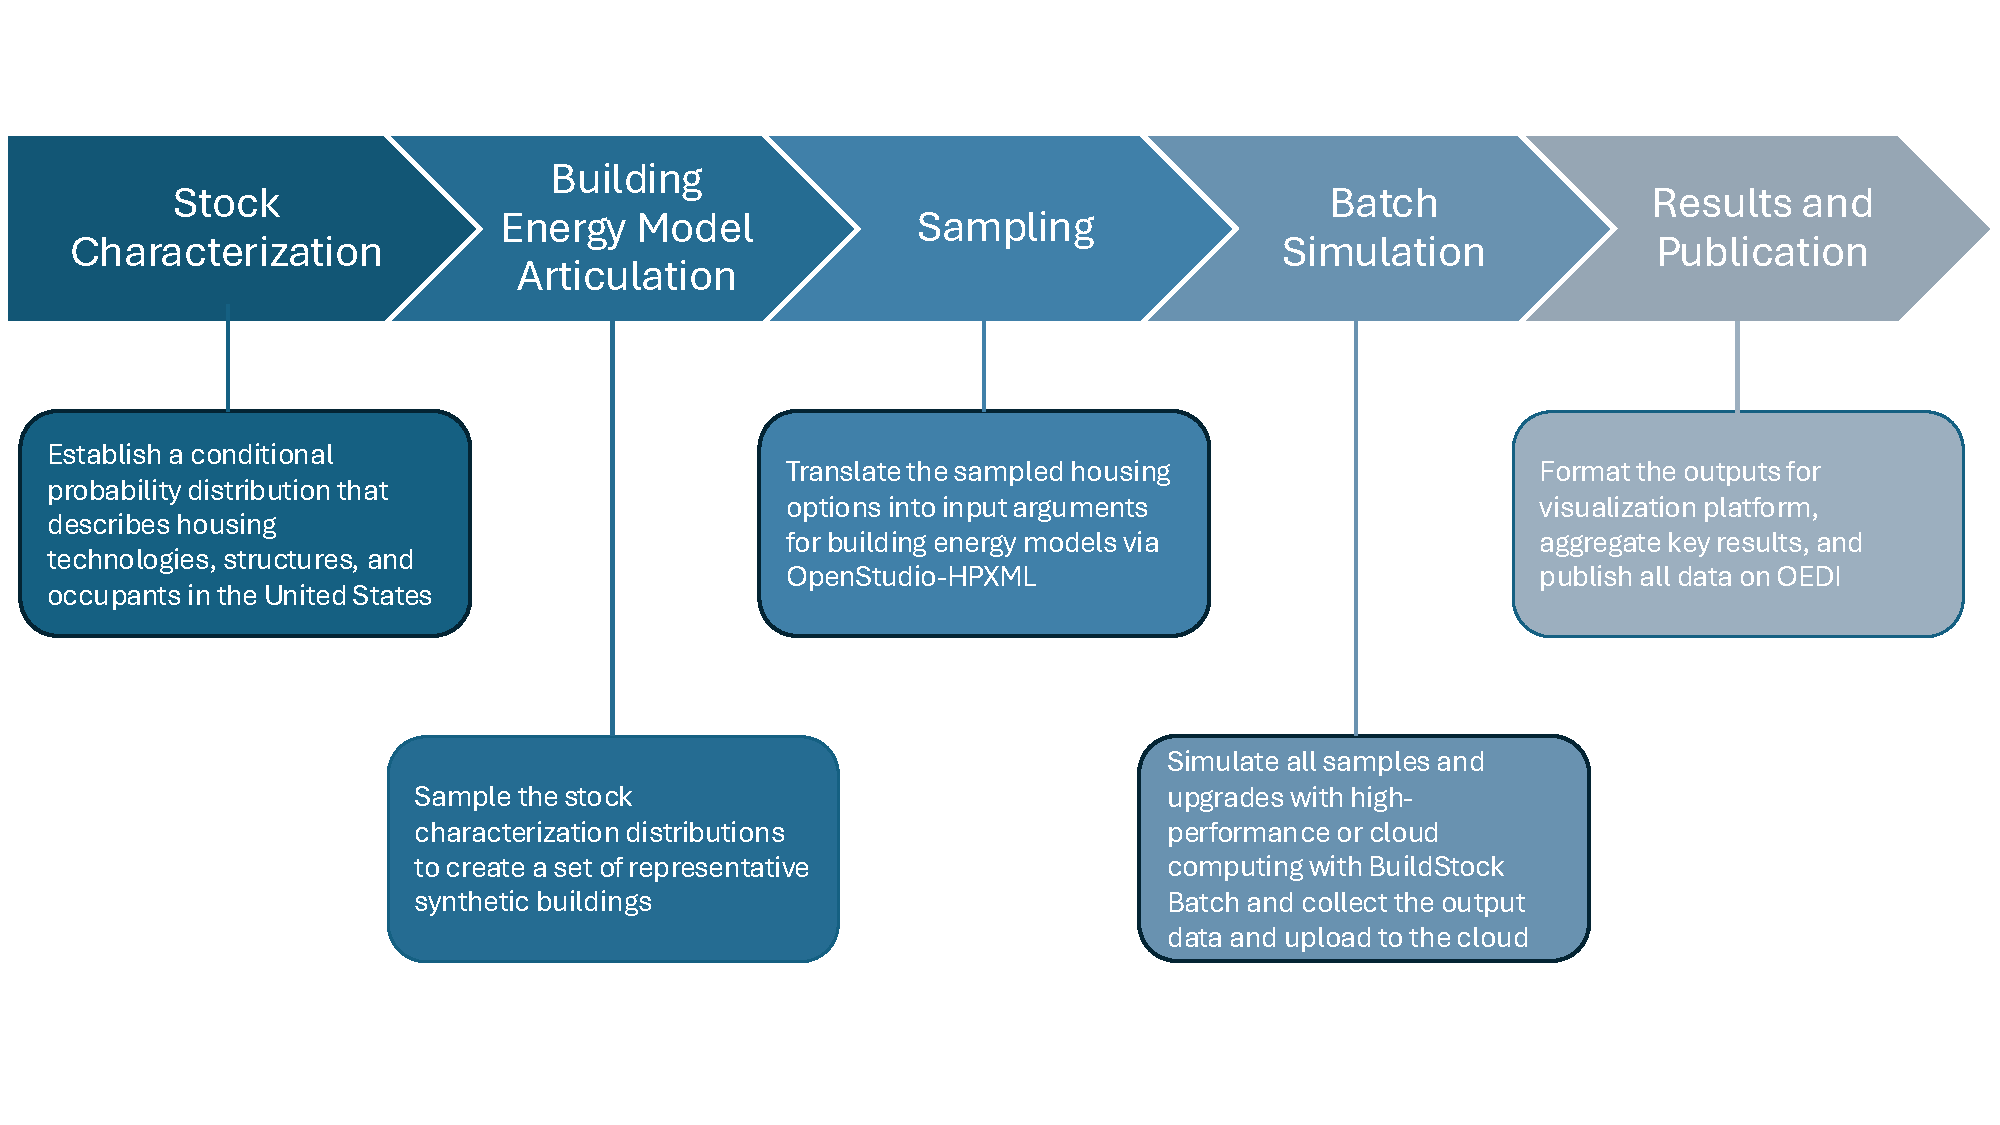
\includegraphics[width=1\linewidth]{images/Figure 1.pdf}
    \caption{A high-level overview of the ResStock workflow steps and what occurs during those steps}
    \label{fig:workflow_overview}
\end{figure}

\section{Stock Characterization}
ResStock characterizes the U.S.~residential building stock and the associated occupants using a probabilistic representation of building and household characteristics developed using the best available data. Much of the underlying data for the U.S.~residential stock comes from national survey data. These surveys include the \href{https://data.census.gov/}{U.S.~Census}, the \href{https://www.census.gov/programs-surveys/acs/microdata.html}{Public Use Microdata Sample} (a microdata version of the American Community Survey [ACS]), the \href{https://www.census.gov/programs-surveys/ahs.html}{American Housing Survey (AHS)}, and the EIA's \href{https://www.eia.gov/consumption/residential/}{Residential Energy Consumption Survey (RECS)}. These surveys provided weighted survey samples with different building characteristics (for example: heating fuel, vintage, number of occupants, floor area, etc.) that ResStock leverages.

ResStock takes this survey microdata, processes it, and connects it to other surveys to develop housing characteristic probability distributions. 

%An example result of this process is the Vintage characteristic distribution of the housing units in the United States. This distribution shows when residential housing units were built in the United States:
%\begin{itemize}
%    \item 13\% of residential housing units were constructed before 1940
%    \item 15\% were constructed between 1940--1959
%    \item 26\% were constructed between 1960--1979
%    \item 27\% were constructed between 1980--1999
%    \item 14\% were constructed between 2000--2009
%    \item 5\% were constructed since 2010
% \end{itemize}
 
%Within each vintage bin, we specify additional distributions of over 150 different characteristics in ResStock. 

Some of these characteristics include the location of the housing unit (examples: state, county, climate zone), the geometry of the housing unit (examples: building type, foundation type, floor area, number of floors), the envelope information (examples: wall insulation, attic type, window panes), appliances (examples: age of refrigerator, heating fuel of the cooking range, whether the unit has in-unit laundry), heating ventilating and air-conditioning (HVAC) system (examples: heating system type, cooling system type, setpoint temperatures, whether the housing unit has ducts), water heating (examples: water heating fuel, type of water heater), household information (examples: income, number of occupants, and tenure). ResStock only contains discrete distributions, and even continuous variables like vintage or floor area are discretized into bins. A given discrete bin of the distributions is referred to as an ``option'' of the characteristic. For example, in the Foundation Type characteristic, there is an option for the unit to have an ``unheated basement'' and another option for the unit to have a ``heated basement.'' Another example is that the Geometry Floor Area characteristic has an option for a housing unit to have a floor area between 1,000 and 14,999 ft\textsuperscript{2}.

%%%%Future improvement - add table of example ResStock characteristics

The input distributions also capture important correlations between building characteristics, sometimes referred to as conditional dependencies. For example, in Los Angeles, CA, in the 1960s, many residential buildings were constructed, while other cities may have seen growth at different periods. This is captured in ResStock by making the Vintage characteristic conditionally dependent on the location of the housing unit, so different locations will have different distributions of housing age. Another example is that energy codes became more widespread in the late 1970s, causing minimum insulation values in new homes to increase. This relationship is captured by making the Insulation characteristics, like wall insulation, conditionally dependent on vintage. Through these correlations taken from the survey data, a network of characteristics and conditional dependencies are assigned through ResStock characteristic variables. It is these conditional dependent distributions of the characteristics that create the residential building stock characterization in ResStock. Information about how these distributions are created can be found in Section \ref{hc_overview}. Detailed information about each characteristic, assumptions, dependencies, and data sources can be found in Section \ref{sec:resstock_inputs}.

\section{Sampling}
ResStock does not model actual buildings (for example: the apartment complex at 123 Main Street). Instead, the housing characteristic distributions are sampled hundreds of thousands of times---typically 550,000---to create a synthetic stock representation of U.S.~housing units. Each sampled housing unit is assigned an option for each of the ResStock housing characteristics. Within the ResStock workflow the full set of sampled housing units and their associated characteristics is referred to as the \texttt{buildstock.csv}. An illustrative example of some characteristics of a ResStock model is shown in Figure \ref{fig:illustrative_sample}. More information about how the sampling is performed can be found in Section \ref{sec:sampling_methodology}. Each of the 550,000 representative samples in the \texttt{buildstock.csv} can be thought of as an archetype residential housing unit description, meaning that each synthetic building represents approximately 250 real U.S.~housing units.

\begin{figure}
    \centering
    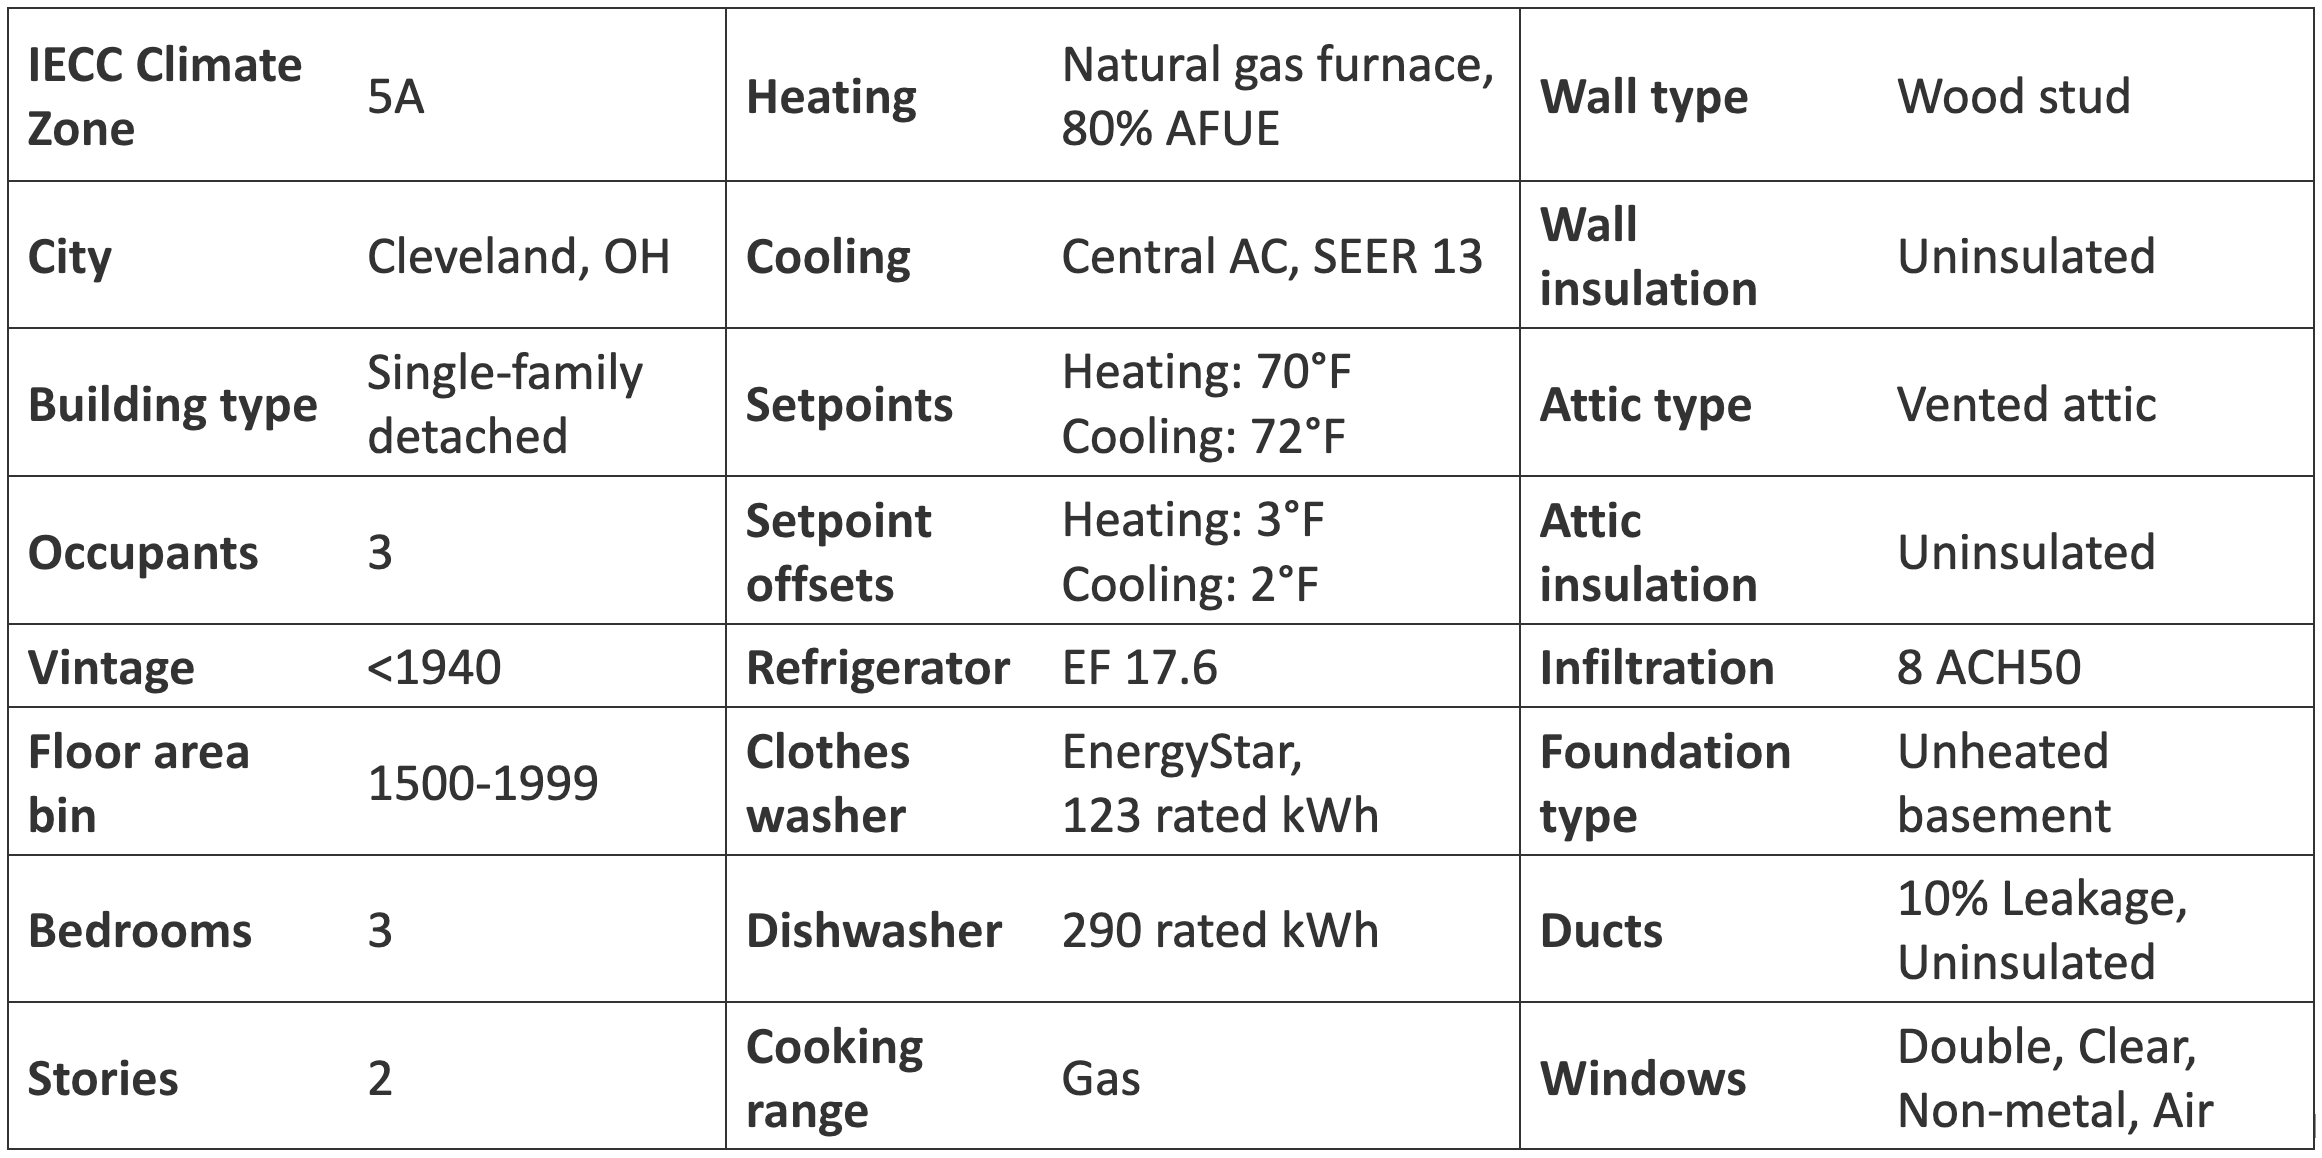
\includegraphics[width=1\linewidth]{images/illustrative_sample.png}
    \caption{An illustrative example of a representative housing unit sample from ResStock (does not show all characteristics available in ResStock)}
    \label{fig:illustrative_sample}
\end{figure}

\section{Building Energy Model Articulation} \label{sec:bem_articulation}
After sampling is complete, the \texttt{buildstock.csv} file contains the synthetic housing stock, with each row representing a sampled housing unit and each column corresponding to a characteristics and the field within that column representing a sampled option. Each housing characteristic has an option assigned for each sampled housing unit in the synthetic stock. The table itself is a set of string values that need to be transformed into a building energy model for each sampled housing unit. The transformation of a single line of characteristic options (see Figure \ref{fig:illustrative_sample} for an example) into an EnergyPlus building energy model is referred to as the model articulation process.

ResStock can be run either just for ``baseline'' energy use---i.e., energy use in the present-day housing stock---or with ``upgrades'' that will simulate both the baseline as well as a technical potential of different technologies to change energy use and associated metrics. The foundation of each of these workflows is the model articulation process. This document discusses primarily the ResStock baseline state since each public data release of upgrade measures has its own accompanying detailed technical documentation. 

% Option lookup, map options to arguments
The first step in the model articulation process maps the options for each housing characteristic within a single row of the \texttt{buildstock.csv} to ResStock modeling arguments. For reference, the mapping is specified in the \href{https://github.com/NREL/resstock/blob/v3.3.0/resources/options_lookup.tsv}{options\_lookup.tsv} file. This file contains all the housing characteristics and all the housing characteristic options in the ResStock national residential stock characterization and the associated ResStock model arguments. This file also includes housing characteristic options that are not sampled in the ResStock baseline, but which could be applied as upgrade options. A list and description of all the ResStock arguments can be found on the \href{https://github.com/NREL/resstock/tree/v3.3.0/measures/ResStockArguments}{ResStock GitHub Repository}. For ResStock to model any option, either in baseline or in upgrade, that option must exist as a \texttt{characteristic | option}  pair in the associated \textit{options\_lookup.tsv}. For example, if there exists a pair \textit{Windows|Double, Clear, Non-metal, Air}, that is then available for use in the baseline housing stock distributions and in upgrade specifications in the project specification file. A \texttt{characteristic | option} pair does not need to exist in the baseline to be used in an upgrade. The technical details associated with each option of the housing characteristics are defined in the \href{https://github.com/NREL/resstock/blob/v3.3.0/resources/options_lookup.tsv}{options\_lookup.tsv} file. For example, the wall exterior finish option: Wood, Medium/Dark is translated into a medium dark color wood siding with an exterior finish R-value of 1.4 in the ResStock measure, which is transformed into other model file inputs. While the ResStock housing characterization provides many inputs that ultimately make up a building model sample (see Section \ref{sec:bem_articulation} for model articulation), it’s important to recognize that there are far more technical details that are not characterized by ResStock, e.g., how much windows are being shaded, how much natural ventilation is used over the course of the year. Instead, these parameters assume the default values from OS-HPXML. For more details on modeling assumptions, refer to the \href{https://openstudio-hpxml.readthedocs.io/en/v1.8.1/}{OS-HPXML documentation} and Section \ref{sec:resstock_inputs} on how building systems are modeled.

Many housing characteristic options are directly used in the creation of the EnergyPlus models, but some are just structural in developing the probability distributions. For example, the ASHRAE IECC Climate Zone 2004 characteristics set the \texttt{site\_iecc\_zone} and \texttt{site\_type} ResStock arguments (Section \ref{sec:ashrae_2004_tsv}), but Location Region is just used as a dependency to define other characteristics that impact the energy modeling. Housing characteristics that do not assign an argument are called meta-parameters, for example Federal Poverty Level. These meta-parameters are often used as intermediate dependencies in other characteristics to separate key housing characteristics that influence the energy simulation. For example, the Federal Poverty Level characteristic and options are used to correlate income to appliance ownership and efficiency. The options and arguments for each ResStock housing characteristic are discussed in detail in Section \ref{sec:resstock_inputs}. 

\subsection{OpenStudio--HPXML}

% ResStock arguments to OpenStudio-HPXML arguments, the HPXML file, class abstraction of the HPXML schema, creation of HPXML file, and the translation of the OpenStudio model.
The next step in the workflow is converting ResStock arguments to the OpenStudio-HPXML arguments to create the HPXML file. OpenStudio-HPXML uses a series of OpenStudio measures to generate an EnergyPlus model for each sample based on the building and occupant characteristics defined by ResStock (Figure \ref{fig:os-hpxml}). In many cases, ResStock relies upon the OpenStudio-HPXML default arguments and calculations. The OpenStudio measures called in the workflow are:

\begin{itemize}
    \item \textbf{BuildExistingModel} -- meta-measure that calls on all following measures in the workflow and passes in ResStock files
    \item \textbf{ResStockArguments} -- translates housing characteristics from ResStock into arguments for BuildResidentialHPXML
    \item \textbf{BuildResidentialHPXML} -- creates the HPXML file for ResStock sample and calculates defaults if not provided from ResStock
    \item \textbf{BuildResidentialScheduleFile} -- generates schedules and references the \texttt{schedules.csv} from the HPXML file
    \item \textbf{ApplyUpgrade} -- meta-measure that calls the following measures in the workflow to modify arguments for samples that have upgrade scenarios applied. 
    \item \textbf{HPXMLtoOpenStudio} -- translation of the HPXML file to an OpenStudio model.
\end{itemize}

\begin{figure}
    \centering
    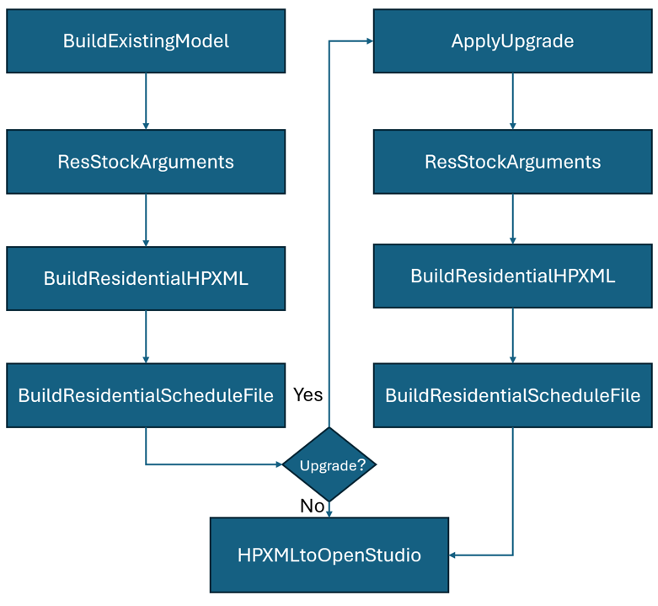
\includegraphics[width=1\linewidth]{images/OSHPXML.png}
    \caption{Flowchart of OpenStudio measures performed to translate a ResStock sample into an OpenStudio model}
    \label{fig:os-hpxml}
\end{figure}

Throughout this translation process, in most cases, the ResStock arguments are the same as the final OpenStudio-HPXML arguments assigned in BuildResidentialHPXML. An example of an identical argument is \texttt{geometry\_unit\_num\_bedrooms}. However, there are some instances where the ResStock arguments intentionally differ from the OpenStudio-HPXML arguments and need further adjustment.  Another potential difference is combining and modifying ResStock arguments into one OpenStudio-HPXML argument. An example is using \texttt{air\_leakage\_percent\_reduction} as part of an envelope upgrade that reduces infiltration. In this scenario, the \texttt{air\_leakage\_value} is adjusted by the \texttt{air\_leakage\_percent\_reduction} argument.

\section{Batch Simulation}
% BuildStock-Batch for the sampling, batch simulation, and post-processing
% Introduce that some parallelization is needed. The computations can either be done on the a local machine, a high-performance computing machine, or even the cloud. A lot of data is produced, post-processing is the biggest memory process.
% The different jobs (sampling/job setup, the array job, and post-processing).
The model articulation process discussed in the previous sections is performed for each of the 550,000 ResStock samples; when factoring in upgrade scenarios, this can result in tens of millions of EnergyPlus simulations. The NREL-developed software \href{https://github.com/NREL/buildstockbatch/tree/v2023.10.0}{BuildStock Batch} manages the various stages of the workflow of running ResStock or ComStock. BuildStock Batch has its own \href{https://buildstockbatch.readthedocs.io/en/v2023.10.0/index.html}{documentation} for a detailed understanding of the software. BuildStock Batch can be run locally, on NREL's high-performance computing (HPC) system, or on the cloud using Amazon Web Services (AWS) or Google Cloud Platform. The local version of BuildStock Batch is mainly used for testing purposes during new feature development and for use in the continuous integration of the ResStock and ComStock software stack. The local version is not used for production-scale runs due to the typically low number of CPU cores and limited memory of local machines. The HPC- or cloud-based workflows can be used to run the full set of baseline samples and upgrade simulations, but all public runs up through 2024 have been completed on NREL's HPC system.

BuildStock Batch is initialized with a project file that configures all the inputs to the workflow. An \href{https://github.com/NREL/resstock/blob/develop/project_national/national_baseline.yml}{example project file} to simulate the national baseline stock can be found in the ResStock repository. There are three major steps to the BuildStock Batch workflow: (1) sample creation and job setup, (2) parallel simulation of all baseline and upgrade simulations, and (3) collection of output data from the simulations and upload to AWS for querying. The sampling and job setup process creates the sampled description of the housing characteristics in the ``buildstock.csv'' file. Then BuildStock Batch submits a job that runs all the simulations in parallel by performing the model articulation and the EnergyPlus simulation for each sample. To run these simulations efficiently, BuildStock Batch communicates with the computing nodes to manage the computing resources at every stage of the workflow. In particular, the software facilitates the simulations in batches by breaking them up into smaller jobs that can be run by parallel processors or by multiple nodes in a distributed manner. This is critical for enabling large-scale simulations which are often time- and memory-intensive to process. BuildStock Batch makes it possible to run hundreds of thousands of simulations in a timely manner by leveraging HPC. After the simulation completes for each model, the workflow post-processes the simulation output by compiling them into annual summary files and coalescing the timeseries into partitioned files separated by upgrade scenario and other user-specified characteristics such as state and county. As the final step, BuildStock Batch can optionally upload the result files to AWS S3 storage, where they can be queried much like a database using web services such as AWS Athena.

A successful run of 550,000 samples with no upgrades, a 15-minute time step, no errors, and no queue time can typically be run on NREL's HPC system within a few hours and creates about 500 GB of output. 

\subsection{Upgrade Specification}\label{sec:upgrades}
In ResStock, most of the details of upgrade specification occur directly in the project file under the \href{https://buildstockbatch.readthedocs.io/en/v2023.10.0/project_defn.html#upgrade-scenarios}{upgrades key}, using fields from the \texttt{options\_lookup.tsv} file specified in logic blocks. Options specified for upgrades include which segment of the baseline the upgrade should be applied to, cost multipliers, and the ``reference'' case, which is important if doing a comparison against a business-as-usual scenario (especially for costs). If the upgrades section is not specified, only the building stock baseline will be simulated. Details of the upgrades associated with each ResStock data release can be found in the supporting upgrade measure documentation.

ResStock upgrades are deterministic, not probabilistic, similar to how the baseline is constructed. You can specify, for example, that all housing units with a specific existing air conditioner in baseline get a specific new air conditioner in upgrade. Or you can use more complex logic and specify 10 different air conditioners in upgrade, based on any characteristic or combination of characteristics. But each housing unit will deterministically receive a specific new air conditioner based on the logic. This can cause challenges. One example is if specifying a new air conditioner for housing units that don't already have air conditioning, you might ideally specify a new, probabilistic range of cooling setpoints for those homes. However, this is not possible. This is why ResStock specifies cooling setpoints for every housing unit, whether or not the unit has air conditioning: so that if an upgrade run assigns air conditioning to that housing unit, the resulting setpoints are appropriately diverse. One can think of this situation as the housing unit's preference of a cooling setpoint if one had a cooling system. There are several other similar parameter option specifications in baseline that are not used to model the baseline but are available in case of certain upgrade option assignments. 

%%%% postprocessing

%%%Need to talk about failed simulations, how they get removed from SDR, and potential implications in representative count (why we say 550k but it's always less than that). How postprocessing sometimes also has to remove buildings with upgrades but no baseline.

\section{Results and Publication}
The results from the BuildStock Batch post-processing include: (1) metadata and annual results (referred to as the \texttt{results.csv} file), (2) a set of end-use timeseries parquet files that combine all the end-use timeseries results from the 550,000 models, and (3) a compressed set of building simulation folders with the results of the OpenStudio-HPXML workflow for each building sample. The \texttt{results.csv} file includes the housing characteristics and annual energy, emissions, utility bills, and cost multipliers for each of the 550,000 models. When a production run of ResStock is completed, reviewed, and ready for publication, the outputs are then reformatted so that each building timeseries is a single file, the result columns start with ``in.<input>'' and ``out.<output>'' (instead of ``build\_existing\_model'' and ``simulation\_output\_report,'' the original outputs of OpenStudio-HPXML), and the energy results are all converted to kWh. This extra step is done in part for readability and ease of use, and also because the \href{https://resstock.nrel.gov/datasets}{ResStock dataset viewer} allows all the energy outputs to be stacked on top of one another and expects the new naming convention. This step is also done outside of the BuildStock Batch workflow. After the conversion, the datasets are uploaded to the \href{https://data.openei.org/submissions/4520}{Open Energy Dataset Initiative End-Use Load Profiles} submission.

\chapter{Input Structure and Sampling} \label{sec:input_structure_and_sampling}
In this section, we discuss the structure of ResStock's input data and our sampling approach. This includes an overview of the probability theory behind ResStock's inputs, how we merge data sources, and how stochastic occupant schedules are created.


\section{Overview of Housing Characteristics} \label{hc_overview}
ResStock uses a set of conditional distributions to describe the characteristics of U.S.~housing units and the households living in them. There are over \href{https://github.com/NREL/resstock/tree/v3.3.0/project_national/housing_characteristics}{150 characteristics described in ResStock}, the majority of which describe the physical attributes of the buildings. Some demographic household characteristics are also included as inputs, both to describe the demographics of the households (e.g., income and renter/owner status) as well as to differentiate key appliance ownership and building characteristic differences that exist between households of different demographics. Each sample in ResStock represents one housing unit (as opposed to a building with many housing units) and will have a value selected for every input housing characteristic defined in ResStock. 

Table \ref{tab:ex_whf_distr} is an illustrative example of a conditional distribution table for the housing characteristic Water Heating Fuel. There are three parts to this table---options, dependencies, and sampling probability. The options are the values a characteristic parameter can take on (e.g., water heater fuel has the options: electricity, fuel oil, natural gas, other fuel, and propane). If one characteristic is described based on another, this is known as a dependency. The dependencies explain how the characteristic is distributed (e.g., Water Heater Fuel saturation varies based on Geometry Building Type RECS, Heating Fuel, and State). Since all buildings must receive a value assigned for a Water Heating Fuel option during sampling, the probabilities in the option columns are equal to one when summed row-wise. Each row gives the parameter distribution within a housing segment defined by the dependencies. For example, the Water Heating Fuel for Mobile Homes with a Heating Fuel of Electricity located in CA has a 72.37\% probability of being Electricity, and a 17.59\% probability of being Natural Gas.  The \textit{sampling\_probability} column provides the likelihood of sampling a home with the dependency characteristics, i.e., the relative size of the housing segment in the United States. The column can be extended with the option probability (i.e., each value under the option column) to give the joint probability of sampling the characteristics of both the dependencies and the option. For example, Mobile Homes with a Heating Fuel of Electricity located in CA represent 0.09022\% of the national residential housing units. Multiplying this by the 72.37\% probability of these housing units having Electricity as their Water Heating Fuel, we determine that Mobile Homes with a Heating Fuel of Electricity located in CA and having a Water Heating Fuel of Electricity represent 0.06529\% of the national residential housing stock.

\begin{table}
    \centering
    \scriptsize
    \begin{tabular}{p{0.2\linewidth}p{0.08\linewidth}p{0.075\linewidth}|
p{0.05\linewidth}p{0.05\linewidth}p{0.05\linewidth}p{0.05\linewidth}p{0.05\linewidth}p{0.075\linewidth}}
    \hline
    Dependency=Geometry Building Type RECS & Dependency=\newline Heating Fuel & Dependency=\newline State & Option=\newline Electricity  & Option=\newline Fuel Oil & Option=\newline Natural Gas & Option=\newline Other Fuel & Option=\newline Propane & sampling\newline \_probability \\
    \hline
    Mobile Home & Electricity & CA & 0.7237 & 0 & 0.1759 & 0 & 0.1005 & 0.0009022 \\
    Multifamily with 2--4 Units & Electricity & CA & 0.6379 & 0 & 0.3621 & 0 & 0 & 0.0026521 \\
    Multifamily with 5+ Units & Electricity & CA & 0.5690 & 0 & 0.4217 & 0 & 0.0093 & 0.0113951 \\
    Single-Family Attached & Electricity & CA & 0.6986 & 0 & 0.2696 & 0 & 0.0318 & 0.0019855 \\
    Single-Family Detached & Electricity & CA & 0.3200 & 0 & 0.6428 & 0 & 0.0372 & 0.0107185 \\
    \hline
    \end{tabular}
    \caption{Subset of Water Heating Fuel distribution}
    \label{tab:ex_whf_distr}
\end{table}

%To illustrate, let’s interpret the last row of Table \ref{tab:ex_whf_distr}. The sampling\_probability tells us that 1.07\% US housing units are single-family detached homes heated using electricity in California. This also means roughly one in 100 models sampled by ResStock will be in this housing segment. The five option columns (starting with Option=) show the probability distribution of water heating in this segment. The probability distribution for Single-Family Detached homes with electric space heating in California has 32.0\% of homes using Electricity for water heating, 0\% Fuel Oil, 64.28\% Natural Gas, 0\% Other Fuels, and 3.72\% Propane. Each of these option probabilities can be multiplied by the sampling\_probability to find the overall likelihood of that option being selected in ResStock. This is known as the joint probability. For example, the joint probability of selecting a Single-Family Detached home with electric space heating in California AND electric water heating is 0.3200 * 0.6528 = 0.34= 0.34\%. This can also be stated that 0.34\% of housing units in ResStock are in California, in Single Family Homes, with electric space heating and electric water heating.

%These dependencies of one housing characteristic on another form a directed acyclic graph in ResStock called the dependency graph. For example, the dependency graph for Bedrooms is shown in Figure \ref{fig:bedrooms_dependency_tree}. The Bedrooms housing characteristic defines the number of bedrooms in the housing unit. On the left side we can see the upstream dependencies of the Bedroom housing characteristic, which are all the characteristics that influence either directly (via a direct dependency) or indirectly (via dependencies further upstream on other nodes) the distribution of the Bedrooms housing characteristic. On the right side, we can see the downstream housing characteristics influenced by the Bedrooms housing characteristic. The color of the nodes indicate the source dataset used to characterize the different nodes in the network (i.e., the data source of the various housing characteristics). In this case, the green nodes come from the PUMS data, which is the microdata version of the American Community Survey, and the black nodes come from the American Housing Survey.  These dependency trees can be interactively generated and analyzed using the \href{https://github.com/NREL/resstock-estimation/blob/develop/utils/dependency_visualizer.py}{dependency\_visualizer} tool in the resstock-estimation repository.
%\begin{figure}
%    \centering
%    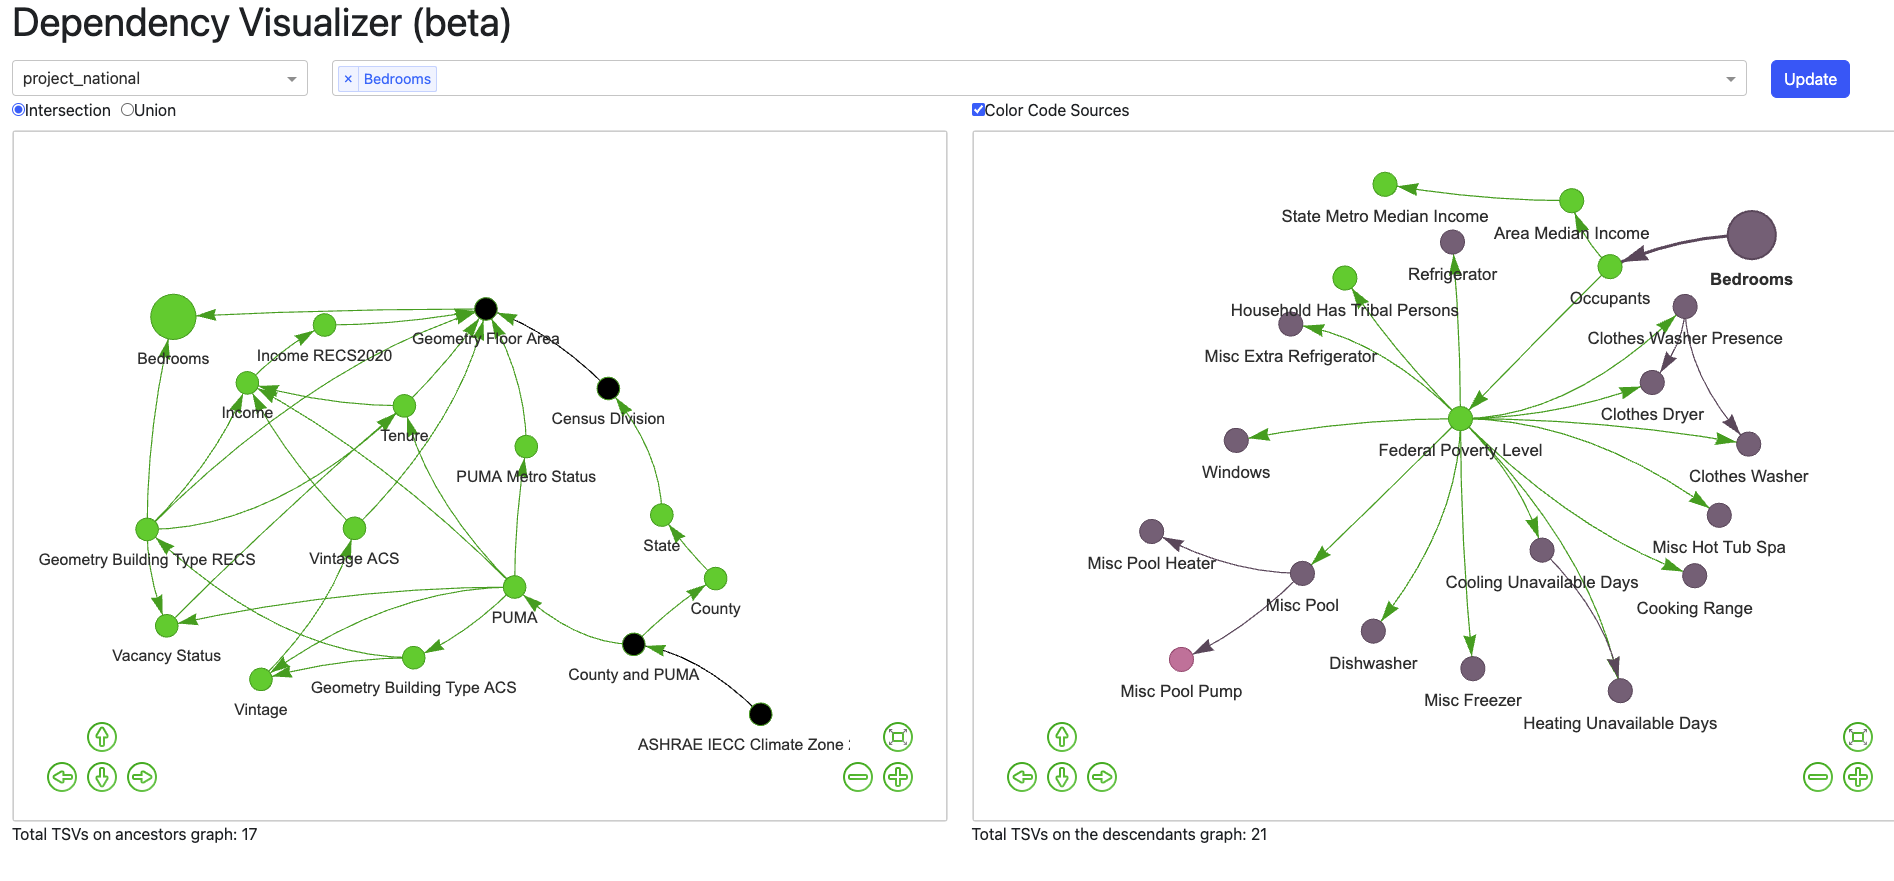
\includegraphics[width=0.9\linewidth]{ResStock Technical Reference Guide/images/bedroom_dependency_tree.png}
%    \caption{Example dependency tree for Bedrooms}
%    \label{fig:bedrooms_dependency_tree}
%\end{figure}

\section{Methods for Creating Housing Characteristic Distributions}\label{hc_method}
ResStock housing characteristics are mostly compiled using publicly available survey data. Major data sources include the Residential Energy Consumption Surveys (RECS) from the EIA \citep{RECS2020}, the Public Use Microdata Samples (PUMS) of the American Community Survey \citep{PUMS}, and the American Housing Survey \citep{AHS}. For certain characteristics that are not yet surveyed nationally, region-specific datasets are used instead. For example, the hot water fixture distribution is informed by field data from a demand management program in the Northeast. Roof insulation, ceiling insulation, and window area characterization come from the Residential Building Stock Assessments by the Northwest Energy Efficiency Alliance \citep{RBSA}. Some housing characteristic distributions are created manually as they do not have any survey data to base on, with about a quarter of ResStock's housing characteristics being constructed using reference numbers from studies. For example, the insulation level for ceilings and walls are derived from the Home Innovation Research Labs 1982--2007 data, and spot ventilation for bathroom and range hood comes from the Building America House Simulation Protocols (\cite{Wilson2014}). Ten characteristics are created based on engineering judgment, including things like door area, plug load diversity, and mechanical ventilation. Each input housing characteristic to ResStock is discussed in detail in Section \ref{sec:resstock_inputs}, including data sources and assumptions. 

ResStock updates housing characteristic distributions to the latest release of longitudinal surveys whenever possible and incorporates new data sources when a need and a data source are both identified. The housing characteristics captured in \href{https://resstock.readthedocs.io/en/v3.3.0/}{ResStock release v.3.3.0} represent the existing U.S.~housing stock as of approximately 2019 (housing stock: {\raise.17ex\hbox{$\scriptstyle\sim$}}2019, weather: 2018 or TMY3, and appliances: {\raise.17ex\hbox{$\scriptstyle\sim$}}2020). ResStock models all 50 states and the District of Columbia. ResStock does not currently model U.S.~territories such as Puerto Rico or Guam.

To generate a housing characteristic's distribution, we generate distributions as normalized cross tabulations of the variables and their dependencies using the sample weight in the source data. We select dependencies from the available variables in the surveys based on a combination of engineering judgment, empirical evidence of correlation, and the need to balance between data fidelity and variability. For example, we know there is likely to be a relationship between having natural gas as a space heating fuel and having natural gas as a water heating fuel since there is already natural gas service to the home, so we set Heating Fuel as a dependency for Water Heating Fuel. Engineering judgment can help pre-select a set of variables to correlate with the parameter. The correlation is then verified with empirical evidence that may include correlation matrices, statistical tests, and plots or tabulations that demonstrate the significance of dependency variables in the output distributions. Input characteristics are constantly being evaluated and updated as better data are identified.

To ensure data fidelity and representativeness, each row in a distribution is generally informed by at least 10 samples in the source data. The number of dependencies to include is limited by the size of the source data, since the data will be sliced over many parameters to generate each row of the distribution. For example, smaller source datasets can afford to split over fewer or less granular dependencies before the data is spread too thin. In such cases, it becomes necessary to choose variables that best capture the variability in the parameter. To do this, we use graph theory and Bayesian inference to calculate the incremental information gain by each candidate variable, which ranks them for selection. Sometimes the dependency selection is further limited to keep the distribution to a manageable file size for workflow purposes. For example, a distribution with a dependency on County will likely have few other dependencies, as doing so will result in an oversized distribution that cannot be stored in the GitHub repository and is otherwise difficult to work with since there are over 3,100 counties in the United States.

In addition to strategic dependency selection, ResStock has two other approaches for dealing with low samples or missing dimensionality in the source data: fallback rules for dimensional coarsening and dimensional blending. Some characteristics in ResStock have several granularity options available, e.g., Vintage (housing unit age grouped into 10 bins) vs.~Vintage ACS (housing unit age grouped into 6 bins). These granularity options help bridge between source data that have different native resolutions to connect the derived distributions. They are also used in fallback rules and dimensional coarsening to address low samples. A common practice in ResStock is to fill the cross tabulation using the native resolution of the dependency variables. Then where there’s insufficient sample count, ResStock pulls the distribution from higher granularity variables to fill the rows. For example, state-level tabulation can be used to fill or supplement the rows with low samples that are natively at the county level. This dimensional coarsening may result in some rows sharing similar probability distributions but at the benefit of filled data gaps and higher sample confidence. The fallback rules are what define these processing sequences so that some or all dependency variables can be coarsened incrementally until all rows reach enough samples. Dimensional coarsening is commonly done over geography, climate zone, vintage, building type, floor area, and income by grouping together similar options or options believed to influence energy consumption similarly (e.g., neighboring geographies). In Section \ref{sec:resstock_inputs} we discuss in the assumptions section for each variable if dimensional coarsening is used.

Another approach to dealing with low samples or missing dimensionality is dimensional blending. This simply refers to updating one distribution with another distribution, hence “blending” the two distributions together. Dimensional blending is often used when a distribution lacks the desired granularity natively and is therefore augmented by another distribution with that granularity. For example, the windows distribution in ResStock comes from RECS, which characterizes the windows based on glass type and frame material. To augment the window options to account for storm window and low-e glazing, the distribution is re-normalized using proportionalities derived from shipment data.

The full cross-tabulation of a parameter and its dependencies can sometimes give rise to impossible or highly improbable combinations of characteristics, e.g., single-family houses that are over 8 stories tall. These combinations are assigned a parameter value of “void,” and prune rules are used in the distribution development to ensure that such combination will never be sampled. If such combination is accidentally sampled (perhaps due to error in upstream housing characteristics), then this will be caught immediately since ``voids'' are supposed to be un-sample-able. Some characteristic combinations are realistic but may be pruned due to limitations in the upstream modeling workflow. For example, in ResStock, single-family detached houses that are 0--1,499 ft\textsuperscript{2} with attached garages can currently only have a single-car garage. This is due to ResStock assuming a specific aspect ratio for building footprint and modeling constraints restricting that the garage cannot be larger or deeper than the livable space.

Many of the housing characteristic distributions are validated by comparing their marginal distribution by each dependency with those of the source data. This is to ensure that any special handling of the data to address low samples or missing dimensionality does not deviate the distributions significantly from the source data. The parity maintained with the source data also means the housing characterization in ResStock inherits the same level of survey biases or uncertainty as those that exist in the source datasets. For example, ResStock’s characterization of Mobile Homes has higher uncertainty than any other housing types as mobile homes are the least common of the major housing types (single-family, multifamily 2--4 units, etc.), and fewer data points exist for them in the source datasets. While using the survey sample weight to construct the distributions helps ensure they are representative of the U.S.~housing stock, ResStock does compare the effect of using different types of sample weight when they are available in certain surveys, such as RECS.



\section{Sampling Methodology} \label{sec:sampling_methodology}
 With the full conditional probability network of inputs defined, ResStock samples the inputs to create the synthetic housing stock. The input file structure and dependency network determine the order in which each characteristic is sampled. Sampling starts with housing features that have no dependencies and next moves to characteristics that have dependencies on the first level of characteristics sampled. This process proceeds until all inputs are sampled and defined. For example, Figure \ref{fig:ex_build_char_distrs} shows an example set of housing characteristic distributions that are interconnected by dependencies. To create a building model in this hypothetical network, the census division is sampled first (and Middle Atlantic is chosen). Then the vintage of the model is sampled based on the distribution of vintage for the chosen census division (1980s is chosen). Next, the heating fuel is sampled according to the distribution for the chosen vintage (natural gas is chosen), and this process repeats until all housing characteristics are determined.  

\begin{figure}
    \centering
    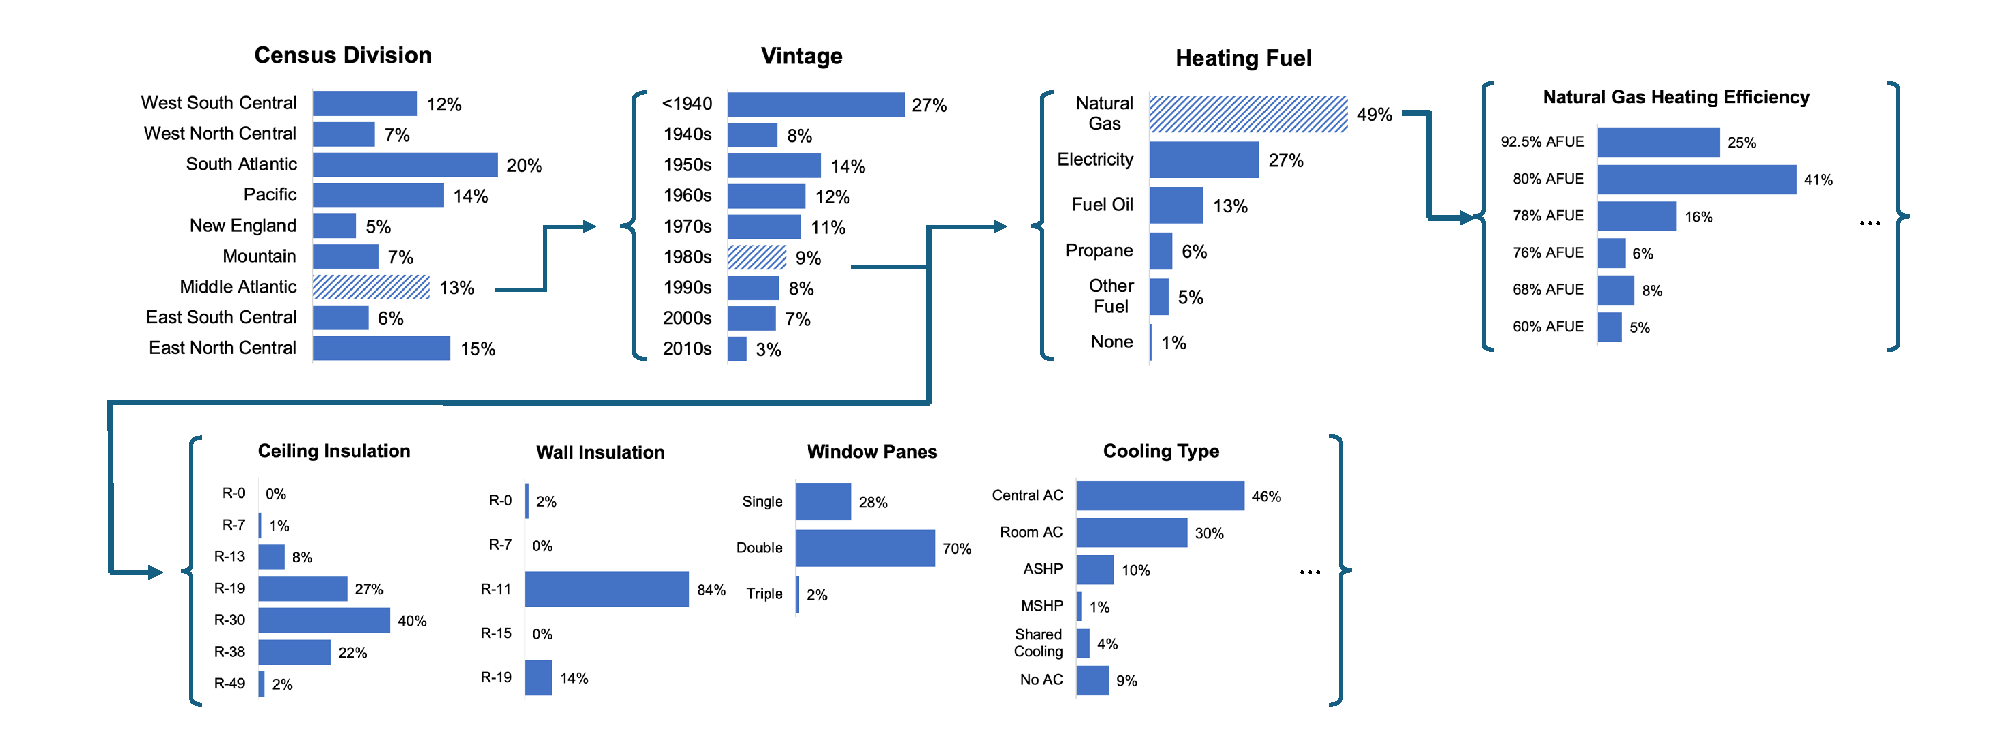
\includegraphics[width=1\linewidth]{images/Figure 4.pdf}
    \caption{Example of interconnected building characteristic distributions}
    \label{fig:ex_build_char_distrs}
\end{figure}

To create a full representative synthetic housing stock for the United States, ResStock employs quota-based sampling. In quota-based sampling, building models are created until the specified number of samples (i.e., the quota) is reached. Sampling starts with the most likely characteristics or most common housing unit in the United States, and then continues filling out increasingly less-likely combinations of characteristics until the quota is reached. This approach creates building models with equal sample weight, meaning each sampled housing unit represents the same number of housing units in the real housing stock. This is a product of quota-based sampling where the likelihood of a building characteristic is directly reflected in the number of times that characteristic is sampled instead of being included in the sample weight.

The quota-based sampling approach is different from purely random sampling (e.g., Monte Carlo) where the samples can come from anywhere in the distributions. Random samples thus may not be representative until many samples are drawn. In quota-based sampling, the quota is multiplied by the probability distributions to determine how many samples will have certain characteristics. If natural gas accounts for 50\% of space heating in the marginal distribution, then one in two samples will be decidedly heated by gas, and this holds true for a quota of two or a quota of a million. However, larger quotas are required to sample uncommon characteristics due to the discretization effect (i.e., a characteristic of 0.1\% probability will not show up in a sampling quota of 500 as 0.1\%*500 = 0.5, which is less than one sample). It is worth noting that the characteristics do not need to be uncommon at the national scale for this problem to occur. Even if a characteristic has 1\% probability nationwide, we will not get the expected 0.01 * 550,000 = 5,500 samples in a national run and in fact may get zero samples if the characteristic has dependencies that will cause it to be sampled within thousands of slices of (quota of) less than 100 samples. While such extreme cases are uncommon, most characteristics do have biases on their national-scale saturation over what one would expect based on the housing characteristic distribution due to this quirk of quota sampling. 

While the diversity in the samples scales with quota in both sampling methods, the rate of reaching a reasonable diversity or converging to the population mean is much faster for quota-based sampling than random sampling. The convergence rate is proportional to the square-root of the quota for quota-based and to the quota for random sampling. The ability to sample for characteristics proportional to their distributions makes quota-based sampling effective as the representativeness of the sampled stock is better maintained even at smaller sampling quotas.

For public datasets, different versions of ResStock runs will by default have different samples. Building model ID 1 is not the same between published datasets.

\section{Schedule Creation}\label{occupancy_model}
In addition to the housing characteristic input files, occupant and energy use schedules are another major necessary building energy model input. Most ResStock schedules are also based upon survey data, but we use a different approach for generating these schedule files since they need to be temporally comprehensive (typically covering a full year with 15-minute time steps) as well as sufficiently diverse to appropriately represent the range of load shapes that occur within the housing stock as well as the aggregate total.

\begin{table}
    \centering
    \scriptsize
    \begin{tabular}{l|l|l|l}
    \hline
    Schedule Name & Unit & Description & Stochastic? \\
    \hline
    \texttt{occupants} & frac & Occupant heat gain schedule & Stochastic \\
    \texttt{lighting\_interior} & frac & Interior lighting energy use schedule & Stochastic \\
    \texttt{lighting\_exterior} & frac & Exterior lighting energy use schedule & Non-Stochastic \\ 
    \texttt{lighting\_garage} & frac & Garage lighting energy use schedule & Stochastic \\
    % \texttt{lighting\_exterior\_holiday} & frac & Exterior holiday lighting energy use schedule. & Non-Stochastic \\
    \texttt{cooking\_range} & frac & Cooking range \& oven energy use schedule & Stochastic \\
    \texttt{refrigerator} & frac & Primary refrigerator energy use schedule & Non-Stochastic \\
    \texttt{extra\_refrigerator} & frac & Non-primary refrigerator energy use schedule & Non-Stochastic \\
    \texttt{freezer} & frac & Freezer energy use schedule & Non-Stochastic \\
    \texttt{dishwasher} & frac & Dishwasher energy use schedule & Stochastic \\
    \texttt{clothes\_washer} & frac & Clothes washer energy use schedule & Stochastic \\
    \texttt{clothes\_dryer} & frac & Clothes dryer energy use schedule & Stochastic \\
    \texttt{ceiling\_fan} & frac & Ceiling fan energy use schedule & Stochastic \\
    \texttt{plug\_loads\_other} & frac & Other plug load energy use schedule & Stochastic \\
    \texttt{plug\_loads\_tv} & frac & Television plug load energy use schedule & Stochastic \\
    %\texttt{plug\_loads\_vehicle} & frac & Electric vehicle plug load energy use schedule. & No \\
    \texttt{plug\_loads\_well\_pump} & frac & Well pump plug load energy use schedule & Non-Stochastic \\
    \texttt{fuel\_loads\_grill} & frac & Grill fuel load energy use schedule & Non-Stochastic \\
    \texttt{fuel\_loads\_lighting} & frac & Lighting fuel load energy use schedule & Non-Stochastic \\
    \texttt{fuel\_loads\_fireplace} & frac & Fireplace fuel load energy use schedule & Non-Stochastic \\
    \texttt{pool\_pump} & frac & Pool pump energy use schedule & Non-Stochastic \\
    \texttt{pool\_heater} & frac & Pool heater energy use schedule & Non-Stochastic \\
    \texttt{hot\_tub\_pump} & frac & Hot tub pump energy use schedule & Non-Stochastic \\
    \texttt{hot\_tub\_heater} & frac & Hot tub heater energy use schedule & Non-Stochastic \\
    \texttt{hot\_water\_dishwasher} & frac & Dishwasher hot water use schedule & Stochastic \\
    \texttt{hot\_water\_clothes\_washer} & frac & Clothes washer hot water use schedule & Stochastic \\ \texttt{hot\_water\_fixtures} & frac & Fixtures (sinks, showers, baths) hot water use schedule & Stochastic \\
    \texttt{heating\_setpoint} & $\deg$ F & Thermostat heating setpoint schedule & Non-Stochastic \\
    \texttt{cooling\_setpoint} & $\deg$ F & Thermostat cooling setpoint schedule & Non-Stochastic \\
    \texttt{water\_heater\_setpoint} & $\deg$ F & Water heater setpoint schedule & Non-Stochastic \\
    \texttt{water\_heater\_operating\_mode} & 0/1 & Heat pump water heater operating mode schedule. 0=hybrid/auto, 1=heat pump only. & Non-Stochastic \\
    % \texttt{battery} & frac & Battery schedule. Positive for charging, negative for discharging. & Non-Stochastic \\
    \texttt{vacancy} & 0/1 & Vacancy schedule. 0=occupied, 1=vacant. Automatically overrides other columns. & Non-Stochastic \\
    %\texttt{outage} & 0/1 & Power outage schedule. 0=power. 1=no power. Automatically overrides other columns. & N/A \\
    \hline
    \end{tabular}
    \caption{Modeled schedules in ResStock}
    \label{tab:schedules}
\end{table}


In ResStock, schedules are used to define a variety of building system operations (Table \ref{tab:schedules}). For example, the space heating and cooling system maintains the indoor air temperature according to a detailed schedule of heating and cooling setpoint temperatures. Interior lighting turns on according to occupancy, while exterior lighting is set to turn on at a specific time frame between the evening and the early morning. These schedules represent either preset equipment schedules, typical usage patterns, or the stochastic time use behaviors of all occupants living within a household. Occupant-driven schedules are typically heterogeneous to represent a diversity of behaviors and preferences. Many of the schedules capture not only the timing of use but also the intensity of use as fractional values, with diversity for every day of the year. These fractional value timeseries are then multiplied by the annual end-use energy or hot water use (calculated separately according to building simulation standards such as ANSI/RESNET/ICC 301 standard or those developed by \cite{bahsp_2010} and \cite{Wilson2014}) to generate the respective end-use load profiles or hot water draw profiles. The schedules are modified for vacant units and vacancy periods (i.e., an occupied household goes on vacation). When a unit is unoccupied for either reason, all schedules are set to zero except for HVAC setpoint temperature schedules designed to keep pipes from freezing. See Section \ref{vacant_units} for more information. In ResStock, schedules are generated either using a stochastic occupancy generator (inherited from OS-HPXML) or through more simplistic defined schedules. %For power outage simulations, all schedules are set to zero except occupancy and general water draws during the periods of the outage. ResStock sets the outage periods via options\_lookup.

\textbf{Stochastic Schedules}. ResStock uses a stochastic schedule generator to produce representative and heterogeneous schedules for occupancy and a number of appliances and hot water end uses. Developed using the \href{https://www.bls.gov/tus/}{American Time Use Survey (ATUS) data from 2013--2017}, submetered appliance energy data, and a supplemental hot water model, the generator combines Markov chain and probability-sampling for schedule simulation. At a high level, the generator uses Markov chain models built from the ATUS data to produce occupant activity schedules for seven different activities: sleeping, personal hygiene, laundry, cooking, dish washing, absent, and active-at-home. These schedules are then processed and combined with appliance information to form household-level appliance and hot water schedules. For example, both clothes washer and clothes dryer events are scheduled to occur during laundry activity, whereas sink events are scheduled to occur during active-at-home activity. More details of the stochastic occupant model can be found in \citet{Chen2022}.

One of the housing characteristics in ResStock is the number of occupants (see Section \ref{occupants} documentation). The generator starts by randomly assigning each occupant within a ResStock model to one of the four preset occupant types that roughly correspond to day-away-evening-home, day-away-evening-away, mostly-home-early-risers, mostly-home-late-risers. These preset occupant types were created by clustering the ATUS data and picking the number of clusters that provides a good balance between clustering performance and diversity of behavior. There is one Markov chain model for each occupant type and for weekday and weekend separately. Each Markov chain model is built from a cluster of respondents sharing a similar occupancy pattern and models their activity progression throughout the day using a time-inhomogeneous activity transition probability. This means what activity happens next depends on both the current activity and the time of day. 

Once the appropriate Markov chain model is picked for an occupant, the schedule generation proceeds with sampling of the starting activity at midnight at the beginning of the weather year and sampling of activity at each time step based on the transition probability given the activity of the previous time step using the Markov-chain transition probability matrix. This process repeats until the full-year schedule is generated for each occupant in the household. Next, the occupant schedules are split into end uses and then merged as a household. The occupant schedules are combined for activities with shareable appliances (e.g., two or more occupants cooking at the same time is one cooking event) and aggregated for individualized activities (e.g., personal hygiene for each occupant is added together for hot water fixtures). While each occupant can only engage in one activity at a time, the activities can overlap after aggregating to the household level. 

Next, the generator converts the household activity schedules into appliance power and hot water schedules. For laundry machines, dishwashers, and range ovens, the generator uses the activity schedules for onset only and samples separately for the duration and power consumption of the appliance, which comes from the 2011 Residential Building Stock Assessment Metering Study (RBSAM) by NEEA. For laundry, the dryer is modeled to start immediately after the washer. For appliance hot water, the activity schedules similarly provide the draw onset while the duration and flow rate are sampled using NREL's Domestic Hot Water Event Schedule Generator~\citep{Hendron2010}. In this way, the hot water schedule and power schedule for the clothes washer and dishwasher are only aligned in terms of the onset and not necessarily the duration. This is consistent with real hot water appliance cycles in which hot water is drawn typically at the beginning. Once an appliance cycle completes with a minimum time gap, the generator finds the next activity onset from the activity schedules and the process repeats until all appliance schedules are created. 

For hot water fixtures, sink use is based on the at-home inactive portion of the occupancy schedule while the personal hygiene schedule is split between shower and bath. For lighting, plug loads, and ceiling fans, circuit-level reference schedules are used and they are modulated by the occupancy schedule. This means the modulated schedule is the same as the reference schedule at 100\% occupancy and ramps down to the minimum of the reference schedule at 0\%. The lighting and plug loads reference schedules are taken from \citet{Wilson2014}, and the ceiling fans' come from RBSAM.  

The stochastic schedule generator produces all appliance schedules at 15-minute resolution and hot water schedules at 1-min to account for their shorter usage duration. These schedules are then aggregated to the simulation time step and then normalized so the maximum demand within a year is 1. The normalized schedules are multiplied by the annual energy or water consumption determined separately for their respective appliances to produce the end-use load profiles. A problem with this modeling approach is that the disconnect between energy calculation and schedule generation can result in unrealistic load profiles, which is especially important when looking at power consumption at shorter timescales. An end-use appliance with a large usage multiplier assigned can also be assigned a stochastic schedule with low usage, thus resulting in unusually large power draws in the simulation and vice versa. This problem is less jarring at the stock level as aggregation tends to balance and smooth out these anomalies. This is an area identified for future improvement.

% For example, the laundry schedule from each occupant is combined to form a single laundry schedule for the household. The laundry schedule provides onset for clothes washer power draw and hot water draw. The power and water draw duration is each sampled separately from supplemental data. The clothes dryer is modeled to start immediately after the clothes washer, with its duration sampled similarly from supplemental data. Once a laundry cycle completes discretely, sampling finds the next onset in the household laundry schedule and the process repeats until the washer and dryer schedules are constructed for the full year. 

\textbf{Non-Stochastic Schedules}. For non-stochastic schedules, ResStock defines various options for 24-hour setback periods (in 1-hour resolution) for HVAC heating and cooling setpoints in options\_lookup. For range spot ventilation (see Section  \ref{range_spot_vent_hour}), the schedule is generated on the fly using inputs that specify the start hour and the number of hours in operation.

There are two types of OS-HPXML schedule input: simple schedule input or detailed schedule input. Simple schedule inputs are available as weekday/weekend fractions and monthly multipliers for a variety of building characteristics. Detailed schedule inputs allow schedule values for every hour or time step of the simulation. They can be used to reflect real-world or stochastic occupancy and must consist of a full year of data, even if the simulation is part-year. The schedule inputs do not need to have the same time resolution as the simulation. They can be more or less granular than the simulation time step. When schedules are not specified, the default OS-HPXML schedules are used. Default schedules can be simple or detailed and are typically smooth, averaged, hourly, and homogeneous schedules mostly derived from Building America House Simulation Protocols (\cite{bahsp_2010}, \cite{Wilson2014}).



